\documentclass[a4paper,10pt]{article}

\usepackage[utf8]{inputenc}
\usepackage[T1]{fontenc}
\usepackage{natbib}
\usepackage[french]{babel}
\usepackage{lmodern}
\usepackage{graphicx}
\usepackage{hyperref}
\hypersetup{
    colorlinks=true,
    linkcolor=blue,
    filecolor=magenta,      
    urlcolor=cyan,
}
\usepackage{microtype}
\setlength{\parskip}{1em}
\usepackage{subfigure}
\usepackage{float}
%\usepackage{url}


\begin{document}

\begin{titlepage}
    \begin{sffamily}
        \begin{center}

%----------------------------------------------------------------------------------------
%	LOGO SECTION
%----------------------------------------------------------------------------------------


\includegraphics[scale=0.6]{images/logo.png}\\[1.5cm]
    
%----------------------------------------------------------------------------------------
%	HEADING SECTIONS
%----------------------------------------------------------------------------------------

\textsc{\LARGE Univérsité de Bretagne Sud}\\[1.5cm]  % Name of your university/college
\textsc{\Large Projet DTN LEPTON-2}\\[1cm]                % Major heading such as course name
\textsc{\large Évaluation de systèmes de communication opportuniste à l’aide de la plate-forme d’émulation LEPTON}\\[0.8cm]  % Minor heading such as course title

%----------------------------------------------------------------------------------------
%	TITLE SECTION
%----------------------------------------------------------------------------------------

    \newcommand{\HRule}{\rule{\linewidth}{0.5mm}} % Defines a new command for the horizontal lines
    
    \HRule \\[0.4cm]
    { \huge \bfseries aDTN vs ibrDTN\\[0.4cm] }
    \HRule \\[1.5cm]

%----------------------------------------------------------------------------------------
%	AUTHOR SECTION
%----------------------------------------------------------------------------------------
    \noindent
    \begin{minipage}{.39\textwidth}
        \begin{flushleft} \large
            \emph{Auteurs:} \\
            Alexandre \textsc{Amouriq} \\
    		Aliyou \textsc{sylla} \\
    		Clément \textsc{Malléjac} \\ 
        \end{flushleft}
    \end{minipage}
    \hfill
    \begin{minipage}{.59\textwidth}
        \begin{flushright} \large
            \emph{Tuteur :} M. Frédéric Guidec \\
            \emph{Responsable :} M. Frederic Raimbault \\
        \end{flushright}
    \end{minipage}
    
    \vfill % Fill the rest of the page with whitespace
    
%----------------------------------------------------------------------------------------
%	DATA SECTION
%----------------------------------------------------------------------------------------
     
    {\large } Promotion 2019-2020\\{Janvier 2020 — Mai 2020}
 \end{center}
  \end{sffamily}
\end{titlepage}

%----------------------------------------------------------------------------
\newpage
%----------------------------------------------------------------------------

\begin{abstract}
L’équipe CASA du laboratoire IRISA mène des recherches sur les réseaux opportunistes.
Dans ce type de réseaux, les équipements mobiles communiquent entre eux sans avoir recours à une infrastructure fixe (points d’accès Wi-Fi, relais 3G/4G...). 
Ils utilisent des transmissions radio directes entre équipements et mettent en place une communication de bout en bout dans le réseau en exploitant les déplacements des équipements qui jouent alors le rôle d’intermédiaires.Dans le cadre de ces recherches, l’équipe CASA a développé une plate-forme d’émulation de réseau mobile opportuniste baptisée LEPTON (Lightweight Emulation PlaTform for Opportunistic Networking). Cette plate-forme mise en œuvre en Java permet d’émuler le comportement d’équipements mobiles, tout en simulant leur mobilité. \par

L’objectif de ce projet est de mener une étude comparative entre deux systèmes de communication opportunistes aDTN et IBRDTN, en utilisant la plate-forme d’émulation LEPTON pour jouer avec chacun de ces systèmes des scénarios de mobilité et de contacts radio. \par

Dans ce rapport, nous présentons les différentes plateformes utilisées. Ensuite nous parcourons les phases de réalisation. Et enfin, nous terminons par la présentation des résultats obetnues suite à l'étude réalisée.
\end{abstract}

%----------------------------------------------------------------------------
\newpage
%----------------------------------------------------------------------------

\tableofcontents

%----------------------------------------------------------------------------
\newpage
%----------------------------------------------------------------------------

\listoffigures

%----------------------------------------------------------------------------
\newpage
%----------------------------------------------------------------------------

\section{Introduction}
Dans le cadre des projets tutorés de M1 Informatique, notre projet porte sur l’évaluation de deux systèmes de communication opportuniste (ibrDTN et aDTN) à l’aide de la plateforme LEPTON. L'objectif est de réaliser une étude comparative entre les deux implémentations du protocole BP (\textit{Bundle Protocol} défini dans le RFC 5050, \cite{rfc5050} des réseaux DTN (\textit{Delay/Disruption-Tolerant Networking}) afin de dégager les éventuelles différences entre elles. \par

Les plateformes ibrDTN et aDTN, développées respectivement par les équipes IBR de l’Université TU Braunschweig et SeNDA de l’Université Autonome de Barcelone, sont des systèmes de communication basés sur les réseaux DTN. Ces types de réseaux utilisent une architecture de bout en bout permettant des communications dans des environnements ayant une connectivité intermittente, des retards importants et/ou variables et un taux d'erreur élevé dans les transmissions. Ils sont initialement conçus pour répondre aux défis de technologies de réseaux capables de faire face aux délais importants et à la corruption des paquets des communications de l'espace lointain. 
Avec l'explosion des objets connectés, les caractéristiques des réseaux DTN sont particulièrement intéressantes pour la mise en réseau de ces objets. Par exemple, le cas des véhicules connectés qui s'échangent des informations sur le traffic ou autres. \par

LEPTON (\textit{Lightweight Emulation Platform for Opportunistic Networking}) est une plate-forme d’émulation de réseaux mobiles opportuniste développée par l’équipe CASA du laboratoire IRISA. Rattachée à l'université Bretagne Sud, l'équipe CASA mène des activités de recherche qui visent particulièrement à soutenir la communication et la fourniture de services dans des réseaux mobiles partiellement ou intermittents connectés. Elle se concentre principalement sur les réseaux mobiles ad hoc et étudie la manière dont l'approche DTN peut aider à soutenir la communication et les services lorsque ces réseaux sont déconnectés. La plateforme LEPTON permet d'émuler le comportement d’équipements mobiles, tout en simulant leur mobilité. \par

Ce rapport est organisé comme suit. Dans la première section, nous présentons les différentes plateformes utilisées dans ce projet à savoir la plateforme d'émulation LEPTON et les systèmes de communication basés sur les réseaux DTN (aDNT et ibrDTN). Après nous parcourons les phases de réalisation dans la deuxième section. Ensuite dans la troisième section, nous discutons des résultats obtenus suite à l'étude réalisée. Et enfin nous terminons par la conclusion et les perspectives. \par

%----------------------------------------------------------------------------
\newpage
%----------------------------------------------------------------------------

\section{Présentation des plateformes utilisées}
Dans cette section, nous présentons les différentes plateformes utilisées pour mener cette étude. La platefome d'émulation LEPTON est d'abord présentée ensuite nous enchainons avec les systèmes opportunistes comparés.

\subsection{Plateforme d'émulation LEPTON}
LEPTON est une plateforme d'émulation  de réseau mobile opportuniste developpée par l'équipe CASA du laboratoire IRISA. Implémentée en Java, elle est distribuée sous les termes de la GNU (General Public License). \par

La plate-forme LEPTON est conçue pour émuler de la mobilité. Principalement utilisée pour l’émulation des réseaux opportunistes. Elle est utile, pour les développeurs qui veulent émuler leurs créations, pour voir de manière simple le résultat de leur travail ainsi que sa validation. Cela permet donc une réelle évaluation d’un système opportuniste. En effet, le point fort de la plate-forme d’émulation de LEPTON, est que sa mise en œuvre ne nécessite pas beaucoup de matériel. Ainsi, l’ordinateur de tous les jours, est suffisant pour sa bonne utilisation. \cite{casa} Il faut tout de même  être doté d’un système d’exploitation Linux.  Par la suite, pour de plus amples utilisations, il est possible d’utiliser LEPTON sur n’importe quel cluster de machine.\par

L’émulation de LEPTON dirige donc les communications entre les instances d’un système opportuniste. Chaque instance détermine ainsi, le comportement d'un nœud du système testé pendant la simulation. Les instances du système opportuniste sont principalement composées d'un code d'application combiné à un middleware de communication, qui lui-même est exécuté sur une pile de protocoles standards. Par la suite LEPTON effectue une succession de transmissions entre ces nœuds, et en fonction de leur position relative \cite{lepton18}.\par

De plus, les instances du système, peuvent être exécutées sur des appareils réels, et offrir de réelles expériences impliquant de vrais appareils, ce qui permet de prouver que le logiciel testé peut fonctionner correctement sur des appareils réels.


\subsection{Systèmes de communication opportunistes (DTN)}

\subsubsection{aDTN}
Développée par le groupe de recherche SeNDA de l'université autonome de Barcelone, la plateforme de communication aDTN (Active-DTN) est une implémentation du protocole BP (\textit{Bundle Protocol}) \cite{rfc5050}. Ce système ouvert et libre (open source) permet de répondre aux besoins de certaines applications de pouvoir spécifier la manière dont leurs messages devraient être traités lorsqu'ils traversent le réseau. Pour cela, il utilise le protocole MMEB (\textit{Mobile code Metadata Extension Blocks}) défini dans le RFC 6258 \cite{rfc6258}, qui permet d'étendre la structure des messages en leur ajoutant d'autres blocs d'informations. Ainsi en plus de la charge utile, les messages transportent également leurs codes de routage, de contrôle de la durée de vie et de prioritisation. Chaque nœud recevant un message exécute ces différents codes afin de décider du traitement à effectuer. Cette décision peut être à quels voisins le message devrait être transféré, s'il devrait être détruit ou avec quelle priorité il devrait être reçu. Implémenté en C++, le système aDTN est distribué avec des bibliothèques permettant le développement des applications DTN avec d'autres languages de programmation très utilisés tels que le C, Java ou Python. \par

L'approche consistant à transporter des codes exécutables dans des messages est très intéressante pour définir le routage de ces derniers et introduire d'autres types de contrôle. Le système aDTN a été conçu pour démontrer la faisabilité de ce paradigme. Plusieurs expériences ont été conduites avec succès sur le campus de l'université autonome de Barcelone (UAB) \cite{lepton18}. \par

Dans cette étude, c'est la version améliorée du système aDTN (aDTNPlus) qui est utilisée. Elle a été adaptée pour avoir une compatibilité avec la plateforme LEPTON. Il est nécessaire de porter une attention particulière à la quantité de ressources globalement consommée pour faire tourner des scénarios dans des bonnes conditions sur des machines relativement limitées en termes de ressource. Pour tenir compte de cette contrainte, le code source a été légèrement modifié afin de réduire la consommation des ressources du système. D'une part, le module qui gère la file d'attente des messages a été modifié pour ne pas sauvegarder sur le disque les messages déjà reçus. Ces messages étaient enregistrés dans le répertoire corbeille de chaque nœud. Et d'autre part, le module procédant au traitement des messages a également été modifié pour éviter de renvoyer un message à un destinateur qui indiquait l'avoir dans sa file d'attente. L'émetteur continuait à renvoyer le message même si le destinateur l'informait qu'il détenait déjà le message dans sa fille d'attente.

\subsubsection{ibrDTN}
ibrDTN est un système opportuniste basé sur l'architecture du protocole bundle, qui est décrite dans le RFC 5050. Cette implémentation est modulaire, car elle peut changer de fonctionnalité par rapport au stockage de bundle tout comme au routage, grâce à ses différentes interfaces. Elle a été conçue pour être embarquée et peut servir pour le cadrage des applications DTN (Delay-Tolerant Networking). \par

ibrDTN est une implémentation C ++ du protocole bundle. ibrdtn a été développé à l’Institut für Betriebssysteme und Rechnerverbund (IBR). Ainsi, IBR-DTN prend en charge les couches de convergences TCP et UDP, le protocole de sécurité de bundle (Bundle Security Protocol) et les spécifications de découverte de voisins IPND (IP Neighbor Discovery). De plus, un support expérimental est également présent pour accéder à un service de dénomination DHT (Distributed Hash Table), pour offrir une embarcation complète du système. Une couche suivant le protocole de communication IEEE 802.15 est également présente, qui est définie par l’IEEE (Institute of Electrical and Electronics Engineers), et qui représente la famille des réseaux locaux : LAN (Local Area Network) et métropolitains : MAN (Metropolitan Area Network), qui sont tous deux basés sur la transmission de données numériques par des liaisons filaires ou sans fil. Les normes IEEE 802 sont plutôt limitées aux réseaux utilisant des paquets de tailles variables contrairement à ceux où les données sont transmises dans des paquets de tailles fixes et courtes. \cite{ibrdtn} \par

Le protocole de communication IEEE 802.15 est donc très adapté pour les réseaux sans fil à faible consommation de débit et de portée, comme pour la famille des LR WPAN (Low Rate Wireless Personal Area Network) par exemple. \par

Le système ibrDTN vise à être très portable et est conçu pour fonctionner sur des systèmes embarqués minimalistes, comme OpenWrt.\par

Il a été testé avec succès sur la famille des processeurs x86,  mais également sur différentes architectures et diverses plates-formes commes MIPS et ARM. Mais encore, ibrDTN prend en charge les distributions Linux x86 / x64 standard, OS X et les smartphones Android. \par

Le code source et les différents packages de distributions sont disponibles sur la  page du projet ibrDTN (GitHub).


\section {Démarche et réalisation}

\subsection {Recherche des scenarios (mobilité/applicatif)}


Pour évaluer les performances des implémentations, il est important d'avoir une application fonctionnant au-dessus du réseau.
Sur conseil de notre tuteur nous avons limité notre recherche à la plateforme CRAWDAD qui recueille des données récoltées ou générées à propos des réseaux sans fil.
Au final, un seul scénario applicatif semblait très pertinent pour tester un DTN, nous n'avons pas eu l'occasion de l'exploiter lors de nos tests.

LEPTON supporte deux méthodes pour connecter deux nœuds ensemble, en se basant sur la distance entre les nœuds ou en utilisant un historique de contact radio.
Sur conseil de notre tuteur, nous nous sommes concentrés sur les données comportant des données de positionnement.
Il est tout de même important de citer les avantages et les inconvénients des deux types de données.
Les historiques de contacts radios permettent de rejouer des conditions réelles qui ne sont pas prises en compte par l'émulation par positionnement comme les aspects topographiques (ligne de vue, réflexions, atténuation ...).
De plus, les données de positionnement étant souvent réalisés par GPS sont d'une précision limitée et d'une période de rafraîchissement variable, 
les données de positionnement donnent le plus souvent la dernière position connue de l'appareil, 
or si la lecture des données GPS ne permet pas de déterminer une nouvelle position dans l'intervalle entre les deux mesures, la même position risque d'être enregistrée deux fois,
de ce fait les données de positionnement peuvent comporter beaucoup d'erreurs (ou d'incohérences), comme des agents se déplacent à des vitesses impossibles.
En contrepartie, les données de contacts ne permettent pas de modifier certains paramètres de l'émulation comme les conditions d'établissements des contacts radios,
là où des données de positionnement permettent de simuler différentes technologies (Wi-Fi 2.4 Ghz, Wi-Fi 5 Ghz, Bluetooth, LoRa ...).

Certaines contraintes nous sont aussi imposées par la nature même de l'émulation, les données devant être livrées aux adaptateurs en temps réel pour limiter les différences entre l'émulation et la situation réelle.
Nous avons donc privilégié les jeux de données de courte durée (moins d'une heure).
De plus, les scénarios doivent avoir des nœuds persistants dans le temps, les rapides créations ou destructions de nœuds ne se prêtant pas vraiment à l'usage de DTN.
La fréquence d'échantillonnage de la position joue elle aussi un grand rôle,
mais elle peut être interpolée entre plusieurs mesures pour avoir un point toujours plus ou moins en mouvement.

Répondant à toutes ces contraintes, nous avons identifié quelques jeux de données potentiellement pertinents sur la plateforme CRAWDAD.

\begin{description}
    \item[coppe-ufrj/RioBuses] Le déplacement de buses à Rio sur une durée d'un mois et d'un intervalle de rafraîchissement d'environ 1 min
    \item[roma/taxi] Le déplacement des taxis à Rome sur une durée d'un mois et d'un intervalle de rafraîchissement de moins 
    \item[thlab/sigcomm2009] Des échanges de messages.
\end{description}

\subsection {Difficultés rencontrées et solutions apportées}

\subsubsection {Consommation des ressources de la plateforme aDTN}
L'un des problèmes majeurs rencontré durant ce travail était une consommation importante de la mémoire par la plateforme aDTN. Cela avait déjà été souligné par l'équipe précédente qui a travaillé sur le sujet. En effet, plus le nombre de nœuds impliqués dans une simulation était grand plus la consommation était élevée. Le nombre de messages échangés joue également un rôle majeur dans cette équation. \par

Les machines à disposition étant assez limitées en termes de ressources, les scénarios utilisés ont donc été limités/tronqués à un maximum d'une centaine de nœuds dans un premier temps pour tenir compte de
cette contrainte. Finalement, il a été décidé de limiter le nombre de nœuds impliqués dans un scénario à une dizaine de nœuds.  \par

Pour réduire cette consommation, les manipulations suivantes ont été réalisées.\par

\noindent \textbf{La non sauvegarde des messages déjà reçus/trop volumineux :}
 
\noindent Chaque nœud de la plateforme aDTN utilise un répertoire (nommé \emph{trash}) pour y stocker les messages qui sont déjà dans sa file d'attente ou qui sont trop volumineux pour tenir dans cette dernière.
Durant l'exécution des scénarios, c'était surtout les messages ayant déjà bien été reçus par le nœud et qui étaient présents dans sa file d'attente qui peuplaient ce repertoire. La taille des messages envoyés a volontairement été limité au minimum de l'ordre de quelques dizaines d'octets. Avec une taille de \emph{1Mo}, la file d'attente d'un nœud n'a donc pas été pleine durant les tests réalisés. Un nœud pouvant recevoir plusieurs fois le même message, il sauvegardait ces messages qu'il recevait à nouveau. Ainsi, on pouvait avoir plusieurs dizaines de milliers fichiers dans le répertoire \textit{trash} d'un nœud. La sauvegarde d'une telle quantité de fichiers est une des raisons pour lesquelles la consommation en mémoire augmentait rapidement en fonction des nombres de nœuds impliqués et de messages envoyés.

Une directive de la compilation conditionnelle a été ajoutée au code source pour prévenir ce comportement dans le cadre de l'utilisation de la plateforme aDTN avec LEPTON.\par

\noindent \textbf{Limiter le nombre de renvoi d'un message :}
 
\noindent Lors d'une communication entre deux nœuds, lorsqu'un des nœuds envoie un message à l'autre et que ce dernier lui notifie qu'il est déjà en possession de ce message (message présent dans sa file d'attente), le premier nœud continuait à lui renvoyer le même message. Ce comportement en plus de générer beaucoup de logs augmentait la consommation en processeur (CPU).\par

\noindent \textbf{Limiter la production des logs :}

\noindent La production des logs a été limitée au strict minimum pour le besoin du traitement des logs générés par les nœuds. Ainsi, juste les événements de création et de réception des messages sont notifiés dans les fichiers de logs.

\subsection {Outils developpés}
Pour les besoins de cette étude, nous avons développé plusieurs outils notamment des scripts bash permettant de simplifier la procédure de lancement des scénarios avec les deux systèmes ibrDTN et aDTN. D'autres programmes ont également été developpés pour effectuer des traitements d'une part en amont sur les données récupérées à partir de la base de données CRAWDAD et d'autre part sur les logs générés par la plateforme LEPTON et les systèmes de communication opportunistes comparés. \par

Dans cette section, nous présentons les outils qui ont été developpés intervenant en amont et en aval de l'exécution des scénarios. Nous commençons par ceux développés en python et ensuite ceux implementés avec scala.

\subsubsection{Python}

\begin{itemize}
  \item dgs
    \begin{description}
        \item Expose des fonctions permettant de créer des fichiers .dgs respectant la grammaire précisée par \href{http://graphstream-project.org/doc/Advanced-Concepts/The-DGS-File-Format/}{graphstream-project.org}.
    \end{description}
  \item dgs\_cut
    \begin{description}
        \item Extrait une période d'un graphe.
    \end{description}
  \item dgs\_remove\_nodes
    \begin{description}
        \item Limite le nombre de nœuds d'un graphe.
    \end{description}
  \item dgs\_reset\_time\_origin
    \begin{description}
        \item Fait une translation dans le temps de tous les événements du graphe pour que la première se situe à l'instant 0.
    \end{description}

  \item remove\_dup\_timestamp
    \begin{description}
        \item Retire les instructions "st" redondantes.
    \end{description}
  \item node\_creation
    \begin{description}
        \item Crée les instructions "an" en se basant sur les instructions "cn" du reste du graphe.
    \end{description}

  \item hist\_from\_node\_file
    \begin{description}
        \item Crée le fichier .hist en se basant sur les instructions "an" du graphe.
    \end{description}
    
  \item log\_ibrdtn\_out\_to\_log\_adtn
    \begin{description}
        \item Le script permet la transformation des résultats de la sortie des logs de LEPTON des nœuds ibrDTN, vers la sortie de ceux de LEPTON pour aDTN. Ainsi, cela fait partie de la marche à suivre pour pouvoir passer les résultats obtenus par le même analyseur pour les deux systèmes, et ainsi minimiser les erreurs.
    \end{description}
  \item modificateurDeLog
    \begin{description}
        \item Le script permet la transformation des résultats de log de chaque nœud généré par ibrDTN.Cette transformation consiste dans l'extraction unique des informations jugées utiles pour la future comparaison. Par la suite, ces informations sont inscrites dans un nouveau fichier, avec un format compréhensible pour l’analyseur de log.
    \end{description}
  \item analyseurGraph
    \begin{description}
        \item Le script permet l’exploitation des fichiers de sortie de l’analyseur de log pour aDTN et ibrDTN. Il permet également la génération automatique de graphiques, qui vont nous permettre d’exploiter les données. Mais aussi, le calcul de certaines variables comme la moyenne de réception globale et le nombre total de messages non transmis.
    \end{description}
  \item logSorter
    \begin{description}
        \item Le script permet de trier les logs de sortie des nœuds de ibrDTN par catégorie.
    \end{description}
    
\end{itemize}



\subsubsection{Scala}
Parmi les outils développés, trois ont été implémentés avec le langage scala. Ils sont décrits ci-dessous. \par

\noindent \textbf{Analyseur de logs (logAnalyzer)} \par
\noindent Ce programme analyse les logs générés par la plateforme LEPTON et les systèmes aDTN et ibrDTN. Après lecture et traitements des fichiers de logs, il produit des données statistiques sur l'exécution d'un scénario donné. Ces données sont subdivisées en trois grandes catégories. La première dite globale rassemble des informations générales tel que le nombre de messages envoyés, reçus et perdus et la durée de l'exécution du scénario. La seconde fournit des données statistiques sur chaque nœud impliqué dans le scénario. Ces données sont entre autres le nombre de messages reçus par un nœud sur le nombre total de messages qui lui a été envoyé etc... Enfin la dernière catégorie contient des détails sur les messages échangés durant le déroulement du scénario. Le fichier de sortie de ce programme est ensuite utilisé par d'autres outils pour la production des différents graphiques. \par

\noindent \textbf{Générateur aléatoire de scénarios applicatifs (aevtGenerator)} \par
\noindent Cet outil permet de générer un scénario applicatif à partir d'un fichier dgs. Sur la base des données lues, le scénario est produit de manière aléatoire en tenant compte de l'état des nœuds (actifs ou non actifs). \par

\noindent \textbf{Nettoyeur des données de performance (performenceDataCleaner)} \par
\noindent Ce programme effectue des traitements sur les données brutes de performance relevées lors de l'exécution d'un scénario afin de les rendre directement utilisables par les outils de production de graphes. Les données de performance sont obtenues à l'aide d'un script bash qui récupère les données de l'ensemble de processus d'un système DTN (aDTN ou ibrDTN). Cet outil est donc utilisé afin de regrouper et d'organiser ces différentes données. \par

\subsection {Environnement d'exécution des scénarios}
Pour la comparaison, nous avons fait tourner les deux systèmes avec les mêmes scénarios de mobilité et applicatif plusieurs fois en agissant sur la période de beaconing (période de diffusion des annonces par les nœuds pour se faire connaître des voisins). En faisant ainsi varier ce paramètre entre 5 et 40 secondes, nous avons pu observer le comportement des deux systèmes face à la variation de la période des annonces diffusées par les nœuds pour se faire découvrir des voisins. 
Les différentes exécutions ont été éffectuées dans les mêmes conditions (avec le même laptop) afin de guarantir la cohérence des résultats obtenus.

\section {Présentation des résultats}
Dans cette étude, nous nous sommes principalement basés sur le paramètre indiquant la période de diffusion des annonces par les nœuds. Ce paramètre a été pour nous celui qui a donné le plus de données intéressantes. \par

Les données extraites ont été analysées de la manière la plus proche possible. En effet, nous avons fait en sorte que les données de ibrDTN ressemblent au maximum aux données de aDTN, et avec le moins d’altérations de données possibles. Avec cela, nous avons pu extraire les données avec le même programme. Pour ensuite, analyser les sorties de log des deux systèmes de la même façon.\par

Le scénario applicatif utilisé a été généré aléatoirement à partir du fichier dgs qui décrit le déroulement du scénario de mobilité. Il s’agit d’un scénario de mobilité réel qui a été réalisé lors d'une expérience menée par l'équipe CASA à l’université Bretagne Sud. Le scénario dure plus d’une vingtaine de minutes, avec une dizaine de nœuds impliqués. Durant l'exécution, 447 messages sont échangés entre les nœuds. \par

Les données sont séparées en trois groupes correspondant aux 4 variantes du même paramètre. Nous avons ainsi extrait des données pour des périodes de diffusion d'annonces de 5, 10, 30 et 40 secondes.

\subsection {Période de beaconing : 5 secondes}

Premièrement, commençons par l’analyse de recherche de voisin(s) fixée à 5 secondes. Du côté de aDTN, nous avons uniquement 23\% de messages reçus contre 94\% du côté d’ibrDTN. La durée moyenne de réception des messages quant à elle est de 18 secondes pour aDTN et de 73 secondes pour ibrDTN. Ces données sont complétées avec la figure \ref{fig:05_avg_rcv_duration}, qui présente la durée moyenne pour chacun des nœuds. La durée moyenne de réception pour aDTN est inférieure à 40 secondes. Tandis que pour ibrDTN elle est supérieure à 40 secondes. \par

\begin{figure}[h!]
    \centering
    \subfigure[aDTN]{\label{fig:05_avg_rcv_duration_adtn}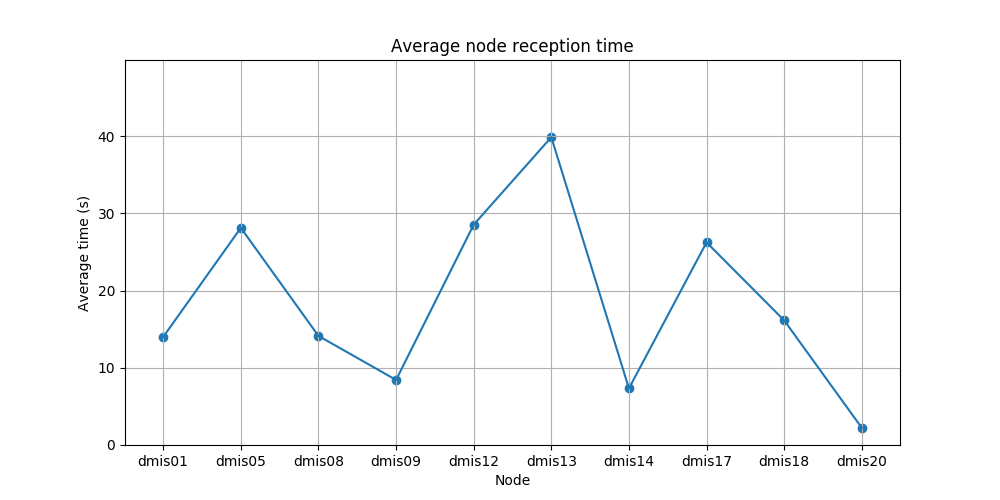
\includegraphics[width=60mm]{images/05/05_avg_rcv_duration_adtn.png}}
    \subfigure[ibrDTN]{\label{fig:05_avg_rcv_duration_ibrdtn}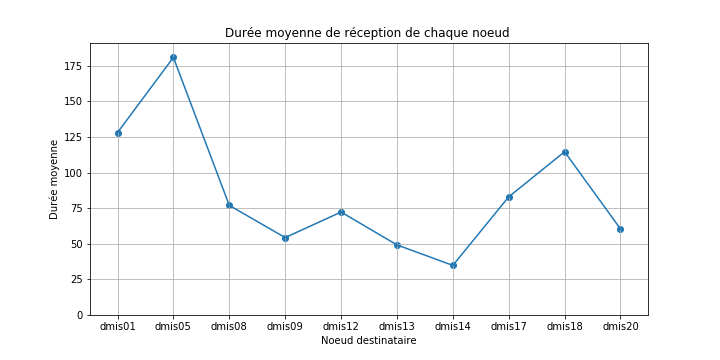
\includegraphics[width=60mm]{images/05/05_avg_rcv_duration_ibrdtn.png}}
    \caption{Durée moyenne de réception par nœud (période 5 secondes)}
    \label{fig:05_avg_rcv_duration}
\end{figure}

La figure \ref{fig:05_avg_snd_duration}, représente la durée moyenne d’envoi de chaque nœud. Celle-ci se situe en dessous de 60 secondes pour aDTN alors que pour ibrDTN elle toujours supérieure à 40 secondes. Ces différents résultats confirment bien pour l’instant les moyennes annoncées plus haut. Ainsi, l’envoi et la réception de messages est plus rapide pour les nœuds de aDTN que pour ceux de ibrDTN. Or, il faut faire attention, car les nœuds de ibrDTN ont envoyé beaucoup plus de messages que ceux de aDTN. En effet, il y a seulement moins d’un quart des messages qui ont été envoyées par aDTN contrairement à ibrDTN. Ainsi, il est normal que la moyenne des messages reçus et envoyés soit plus basse pour aDTN.\par

\begin{figure}[h!]
    \centering
    \subfigure[aDTN]{\label{fig:05_avg_snd_duration_adtn}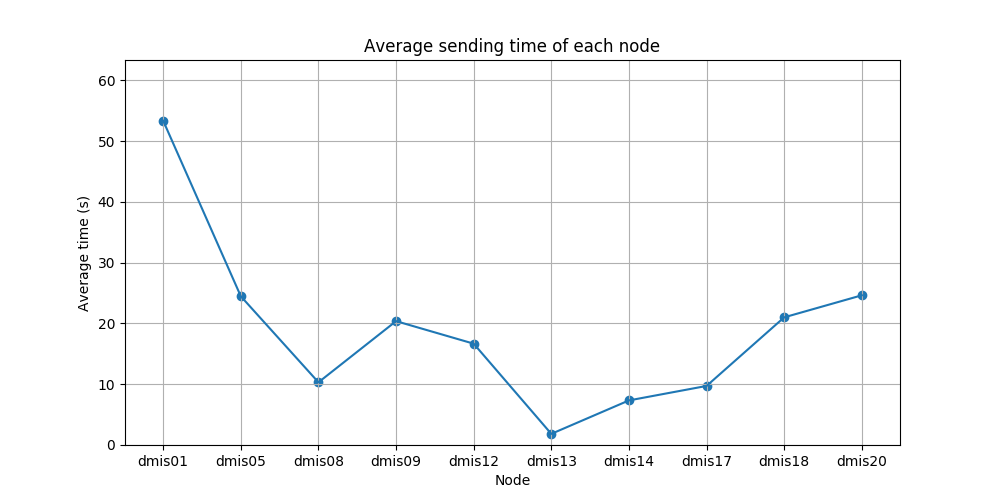
\includegraphics[width=60mm]{images/05/05_avg_snd_duration_adtn.png}}
    \subfigure[ibrDTN]{\label{05_avg_snd_duration_ibrdtn}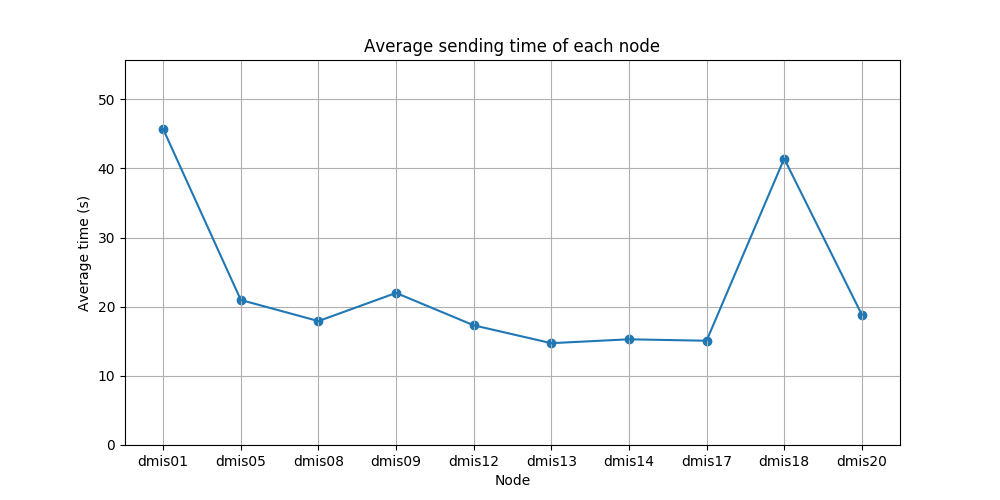
\includegraphics[width=60mm]{images/05/05_avg_snd_duration_ibrdtn}}
    \caption{Durée moyenne d'envoi par nœud (période 5 secondes)}
    \label{fig:05_avg_snd_duration}
\end{figure}

La figure \ref{fig:05_nb_neighbors} présente le nombre maximal et minimal de voisin(s) par nœud. Nous pouvons voir que du côté de aDTN, le nombre maximal de voisins est toujours inférieur à 6. Tandis que pour ibrDTN ce nombre maximal est supérieur à 6. Par contre le nombre de voisin minimal est le même, soit un voisin.\par

\begin{figure}[h!]
    \centering
    \subfigure[aDTN]{\label{fig:05_nb_neighbors_adtn}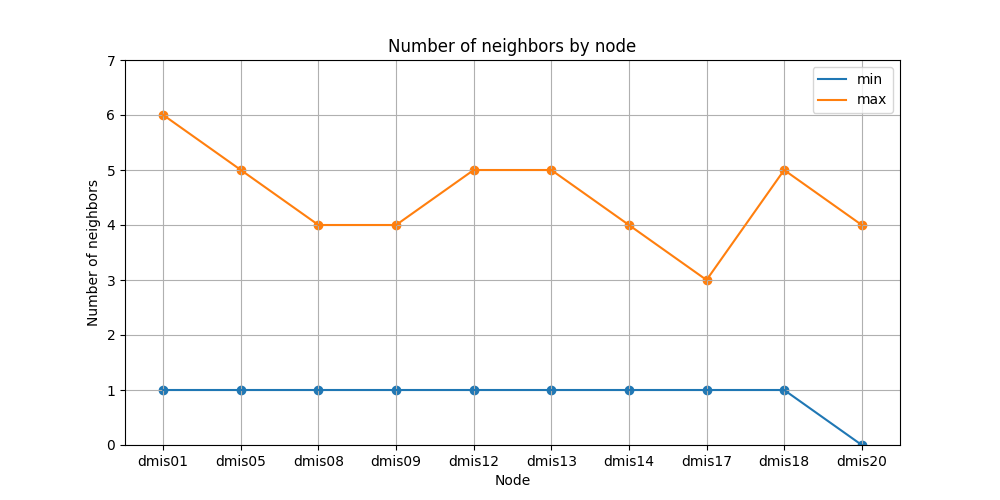
\includegraphics[width=60mm]{images/05/05_nb_neighbors_adtn.png}}
    \subfigure[ibrDTN]{\label{fig:05_nb_neighbors_ibrdtn}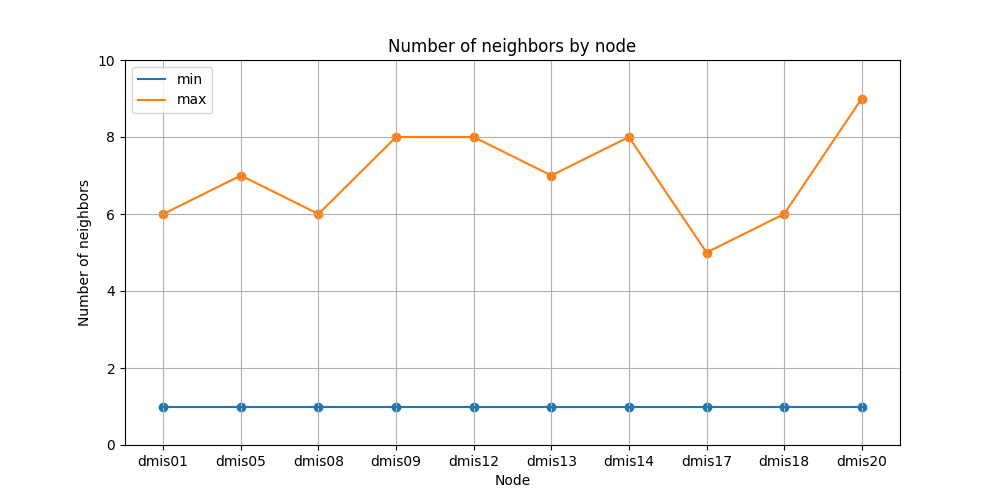
\includegraphics[width=60mm]{images/05/05_nb_neighbors_ibrdtn}}
    \caption{Nombre de voisins par nœud(s) (période 5 secondes)}
    \label{fig:05_nb_neighbors}
\end{figure}

La figure \ref{fig:05_msg_rcv} présente les pourcentages des messages reçus pour chaque nœud. Nous pouvons observer une grande différence, car les nœuds d’ibrDTN reçoivent 100\% des messages comparés à ceux de aDTN, qui ont des pourcentages variés, avec au plus bas 7\% et 35\% au plus haut.\par

\begin{figure}[h!]
    \centering
    \subfigure[aDTN]{\label{fig:05_msg_rcv_adtn}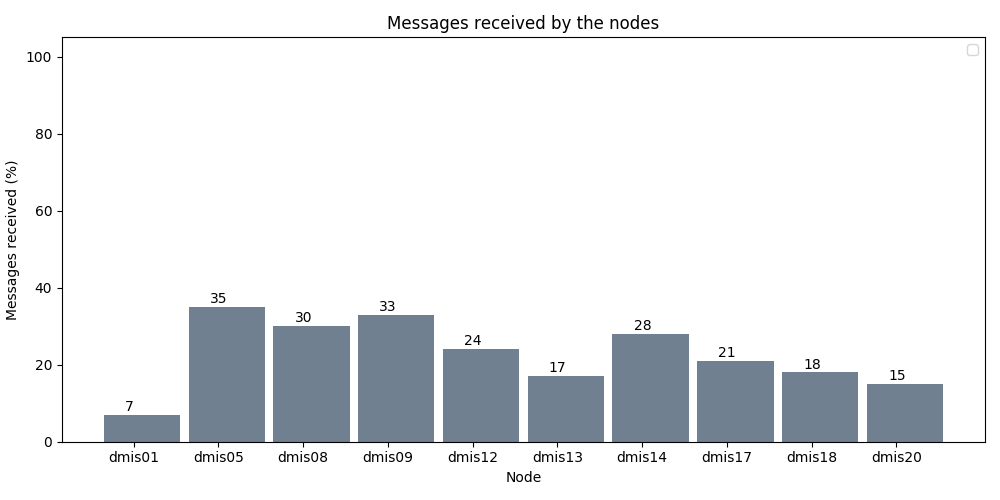
\includegraphics[width=60mm]{images/05/05_msg_rcv_adtn.png}}
    \subfigure[ibrDTN]{\label{fig:05_msg_rcv_ibrdtn}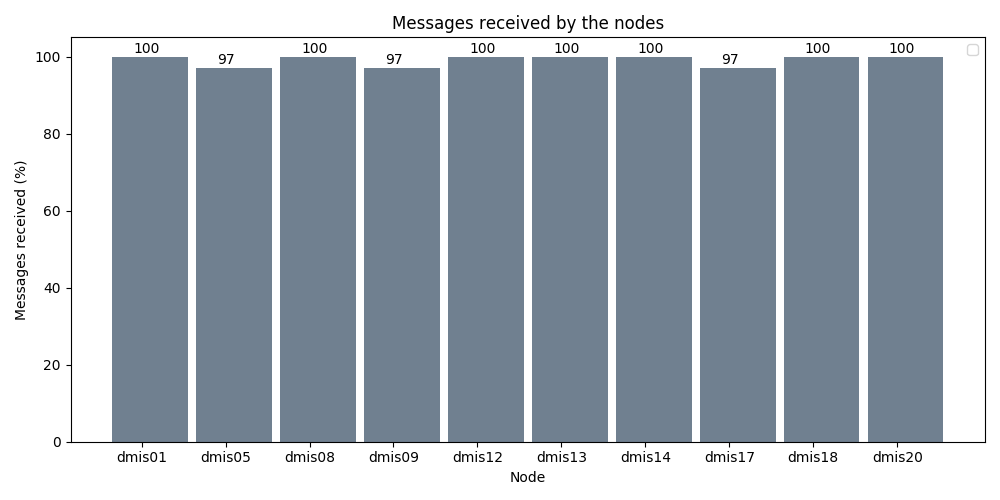
\includegraphics[width=60mm]{images/05/05_msg_rcv_ibrdtn}}
    \caption{Messages reçus par nœud (période 5 secondes)}
    \label{fig:05_msg_rcv}
\end{figure}

Il faut faire attention pour ibrDTN car on pourrait penser qu’il reçoit 100\% des messages, or ce n’est pas le cas. Ce résultat provient du traitement des données, de l'extraction et des soucis pour connaître le créateur du message. Il faut plutôt prendre en compte le nombre de messages non reçus global qui est de 25 contre 343 pour aDTN.\par


\subsection {Période de beaconing : 10 secondes}
Deuxièmement, nous nous sommes intéressés à la recherche de voisin(s) fixée à 10 secondes. Nous remarquons que aDTN reçoit 51\% des messages envoyés alors que ibrDTN en reçoit 94\%. Ainsi, la durée moyenne de réception des messages est de 37 secondes pour aDTN contre 75 secondes pour ibrDTN. Nous pouvons comparer ces moyennes par rapport à la figure \ref{fig:10_avg_rcv_duration} qui présente la durée moyenne de réception des messages par nœud. Pour aDTN, les durées moyennes sont inférieures à 80 secondes alors que pour ibrDTN, elles sont supérieures à 50 secondes. Ainsi, les durées de réception sont, en moyenne, plus élevées pour ibrDTN que pour aDTN.\par

\begin{figure}[h!]
    \centering
    \subfigure[aDTN]{\label{fig:10_avg_rcv_duration_adtn}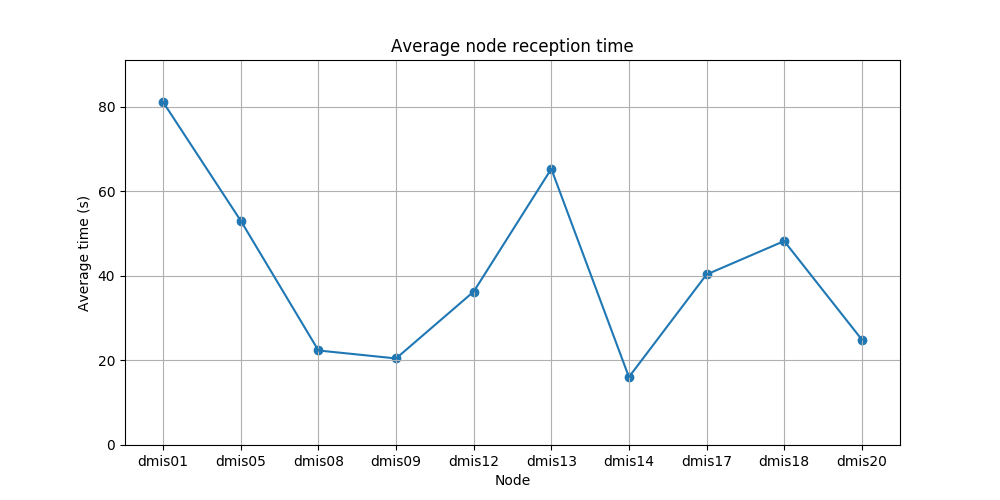
\includegraphics[width=60mm]{images/10/10_avg_rcv_duration_adtn.png}}
    \subfigure[ibrDTN]{\label{fig:10_avg_rcv_duration_ibrdtn}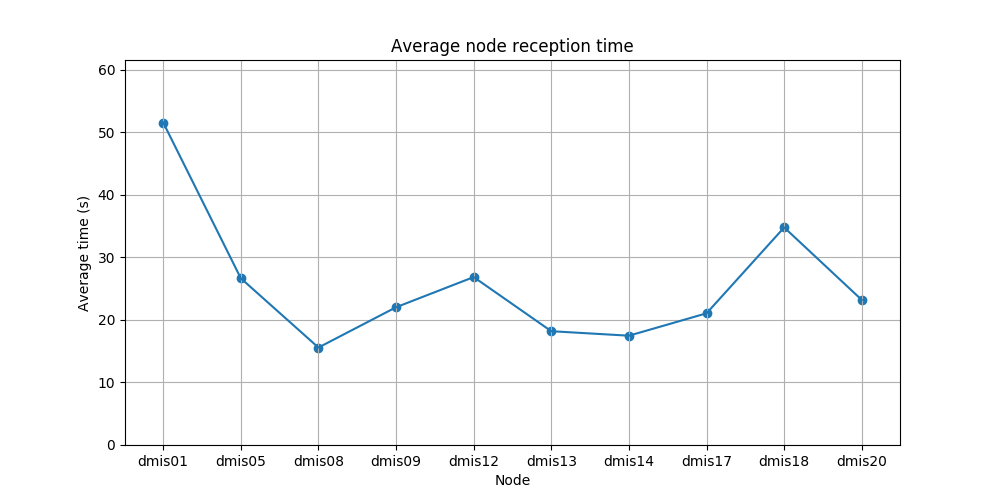
\includegraphics[width=60mm]{images/10/10_avg_rcv_duration_ibrdtn}}
    \caption{Durée moyenne de réception par nœud (période 10 secondes)}
    \label{fig:10_avg_rcv_duration}
\end{figure}

Il est également intéressant de regarder les résultats de la durée moyenne d'envoi de chaque nœud, observable en figure \ref{fig:10_avg_snd_duration}. Les résultats oscillent, pour la majorité des nœuds, entre 20 et 40 secondes du côté de aDTN. Pour ibrDTN, la durée moyenne se situe principalement entre 50 et 100 secondes, soit toujours supérieure à celle de aDTN. Cependant, il faut tenir compte que ibrDTN envoie près du double de messages, et qu’ainsi il y a plus de valeurs, ce qui peut expliquer des moyennes plus élevées. \par

\begin{figure}[h!]
    \centering
    \subfigure[aDTN]{\label{fig:10_avg_snd_duration_adtn}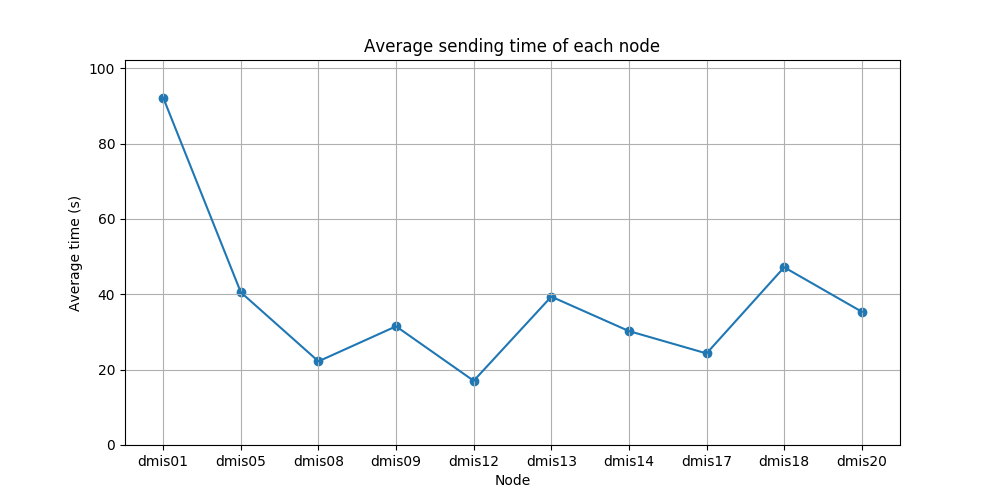
\includegraphics[width=60mm]{images/10/10_avg_snd_duration_adtn.png}}
    \subfigure[ibrDTN]{\label{fig:10_avg_snd_duration_ibrdtn}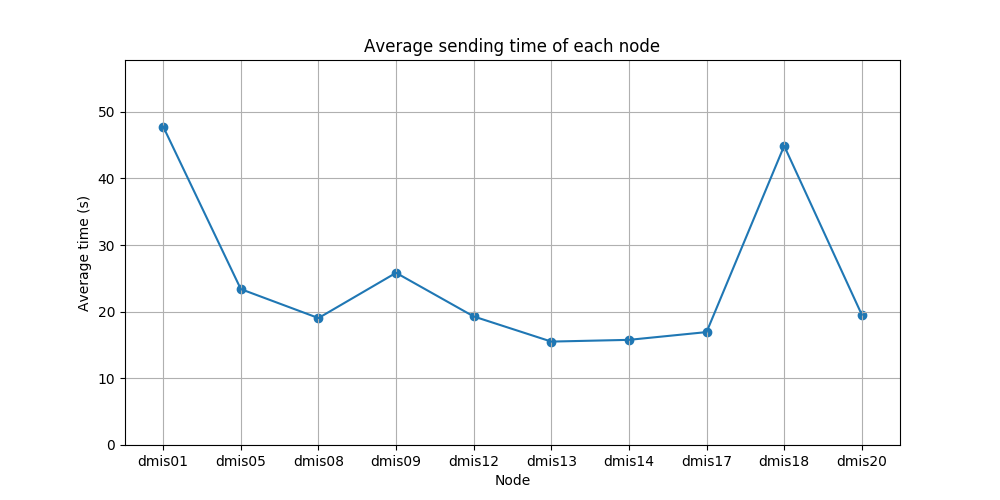
\includegraphics[width=60mm]{images/10/10_avg_snd_duration_ibrdtn}}
    \caption{Durée moyenne d'envoi par nœud (période 10 secondes)}
    \label{fig:10_avg_snd_duration}
\end{figure}

La figure \ref{fig:10_nb_neighbors} montre le nombre de voisin(s) par nœud. Ces courbes permettent d'observer que le nombre de voisin minimal est le même pour aDTN et ibrDTN et il est de un. En revanche, le nombre de voisins maximal est différent. En effet, il est de 5 pour aDTN et pour ibrDTN, il est presque toujours supérieur à celui de aDTN, soit plus de 5.\par

\begin{figure}[h!]
    \centering
    \subfigure[aDTN]{\label{fig:10_nb_neighbors_adtn}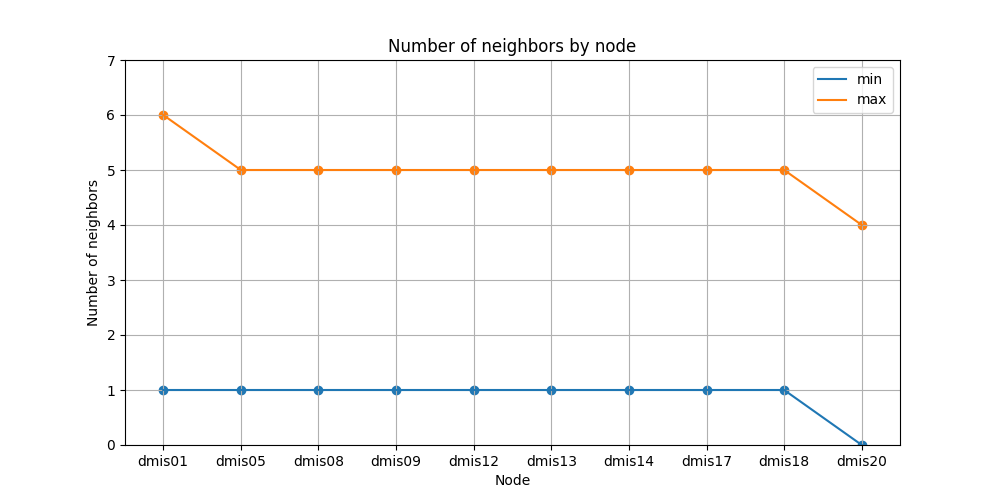
\includegraphics[width=60mm]{images/10/10_nb_neighbors_adtn.png}}
    \subfigure[ibrDTN]{\label{fig:10_nb_neighbors_ibrdtn}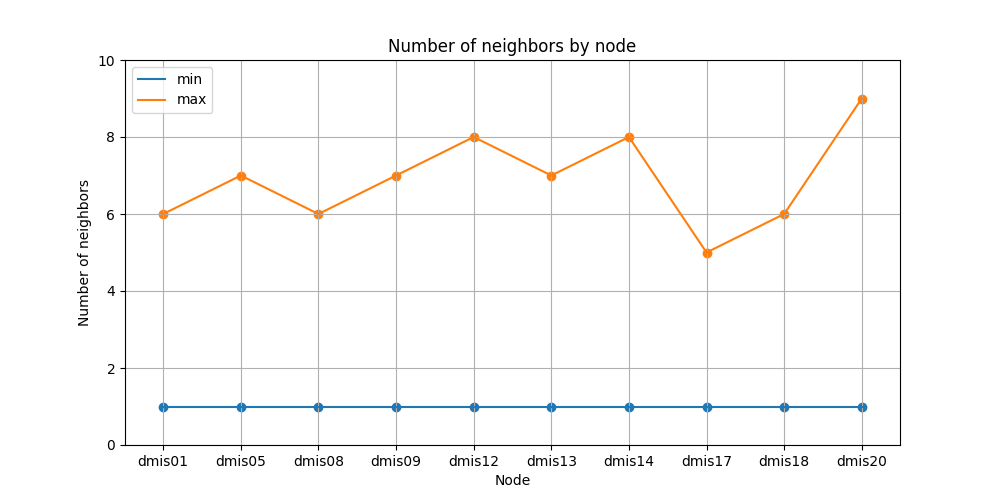
\includegraphics[width=60mm]{images/10/10_nb_neighbors_ibrdtn}}
    \caption{Nombre de voisins par nœud(s) (période 10 secondes)}
    \label{fig:10_nb_neighbors}
\end{figure}

Les diagrammes en barres de la figure \ref{fig:10_msg_rcv}, fournissent les pourcentages des messages reçus pour chaque nœud. Nous pouvons voir une grande différence, car les nœuds d’ibrDTN reçoivent 100\% des messages comparés à ceux de aDTN. Ce dernier système, reçoit quant à lui un nombre très variable de messages en fonction des différents nœuds. Au plus bas, il reçoit 36\% des messages et au maximum il reçoit 73\%. En ce qui concerne ibrDTN, comme expliqué précédemment, nous nous intéressons plutôt au nombre de messages transmis et non reçus. Ainsi, ibrDTN a 25 messages non reçus contre 215 pour aDTN. Par conséquent, ibrDTN reçoit tout de même 9 fois plus de messages.\par

\begin{figure}[h!]
    \centering
    \subfigure[aDTN]{\label{fig:10_msg_rcv_adtn}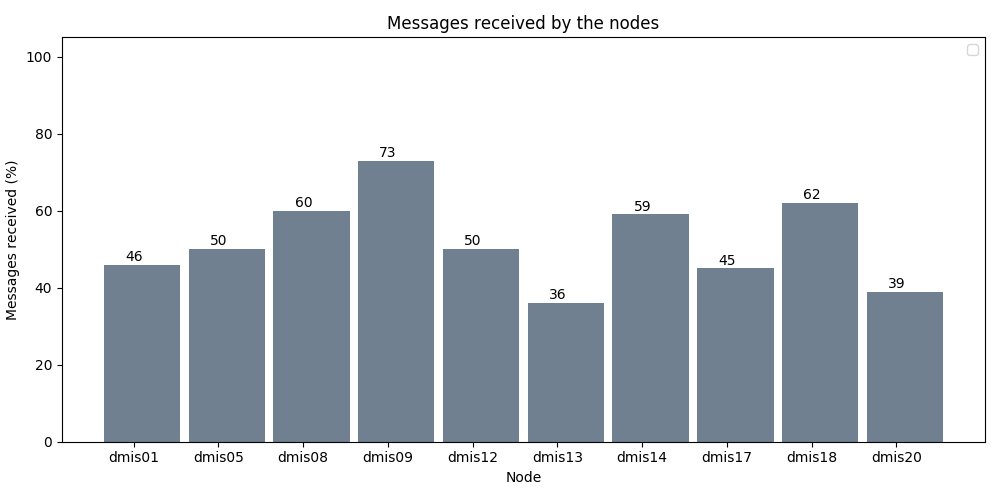
\includegraphics[width=60mm]{images/10/10_msg_rcv_adtn.png}}
    \subfigure[ibrDTN]{\label{fig:10_msg_rcv_ibrdtn}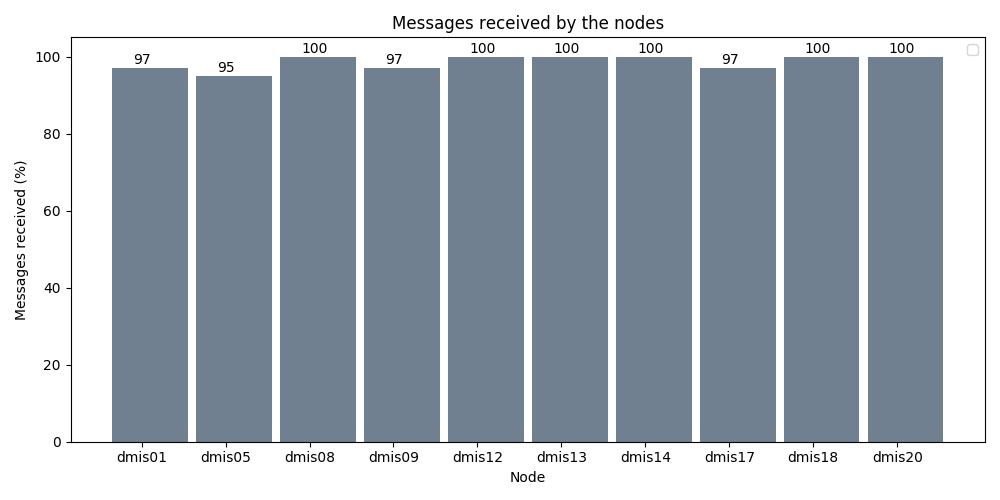
\includegraphics[width=60mm]{images/10/10_msg_rcv_ibrdtn}}
    \caption{Messages reçus par nœud  (période 10 secondes)}
    \label{fig:10_msg_rcv}
\end{figure}


\subsection {Période de beaconing : 30 secondes}
Troisièmement, nous explorons les résultats avec une recherche de voisin(s) fixée à 30 secondes. Tout d’abord, nous avons une moyenne de réception des messages de 68 secondes pour aDTN contre 97 pour ibrDTN. Le nombre de messages reçus est de 98\% pour aDTN et de 90\% pour ibrDTN. Nous pouvons nous intéresser aux graphiques de la figure \ref{fig:30_avg_rcv_duration}, qui montrent la durée moyenne de réception de chaque nœud. Nous remarquons que, pour aDTN, cette valeur moyenne ne dépasse globalement pas les 80 secondes contrairement à ibrDTN. En effet, pour celui-ci, la durée moyenne de réception des messages est supérieure à 60 secondes et atteint même 150 secondes pour les nœuds dmis01 et dmis18.\par

\begin{figure}[h!]
    \centering
    \subfigure[aDTN]{\label{fig:30_avg_rcv_duration_adtn}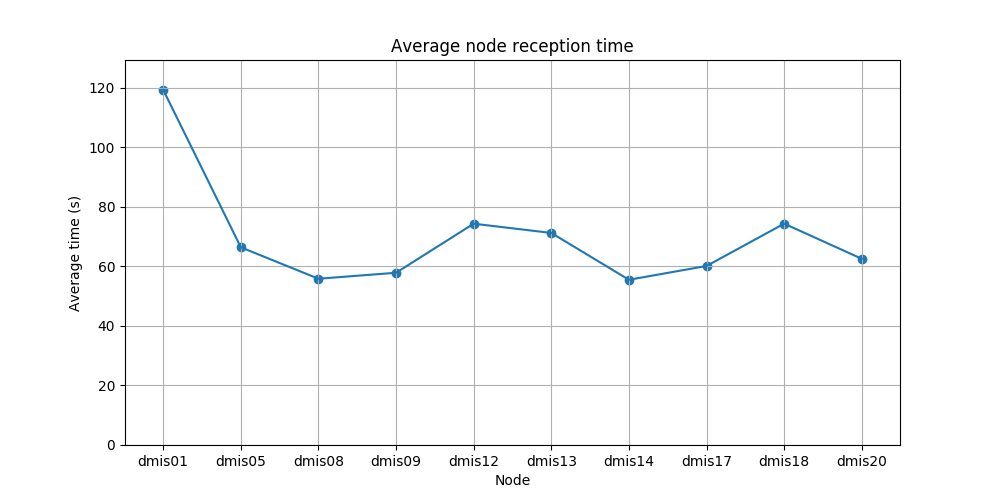
\includegraphics[width=60mm]{images/30/30_avg_rcv_duration_adtn.png}}
    \subfigure[ibrDTN]{\label{fig:30_avg_rcv_duration_ibrdtn}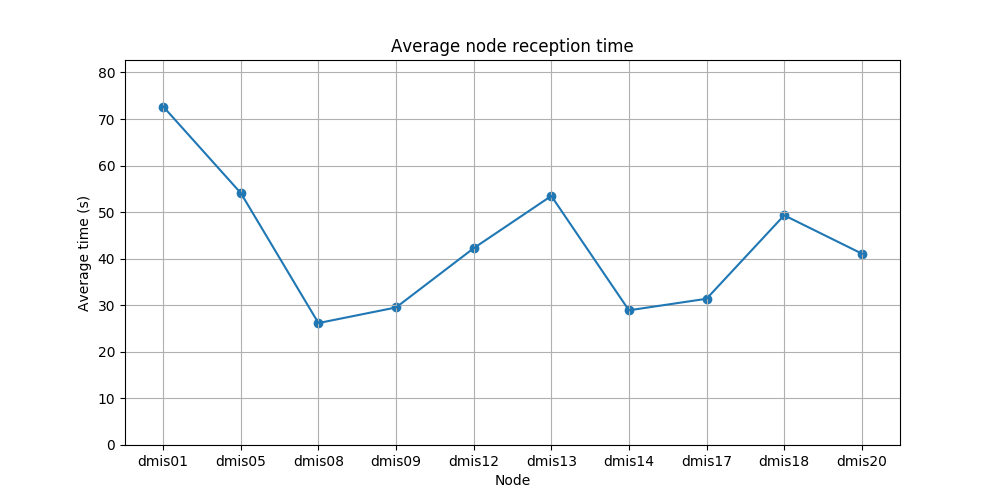
\includegraphics[width=60mm]{images/30/30_avg_rcv_duration_ibrdtn}}
    \caption{Durée moyenne de réception par nœud (période 30 secondes)}
    \label{fig:30_avg_rcv_duration}
\end{figure}

Les courbes représentant la durée moyenne d’envoi de chaque message par nœud de la figure \ref{fig:30_avg_snd_duration}, montrent une certaine différence. En effet, cette durée oscille entre 40 et 80 secondes pour aDTN et 60 et 100 pour le second. Par ailleurs, pour trois nœuds de ibrDTN, il est possible de noter que la durée moyenne est largement plus élevée (supérieure à 135 secondes). La même remarque peut être faite pour le nœud dmis01 du système aDTN.\par

\begin{figure}[h!]
    \centering
    \subfigure[aDTN]{\label{fig:30_avg_snd_duration_adtn}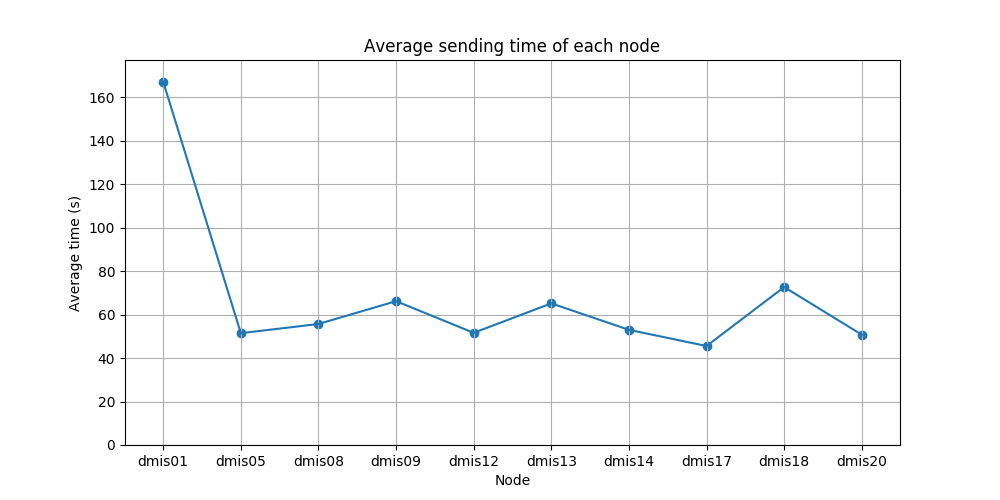
\includegraphics[width=60mm]{images/30/30_avg_snd_duration_adtn.png}}
    \subfigure[ibrDTN]{\label{fig:30_avg_snd_duration_ibrdtn}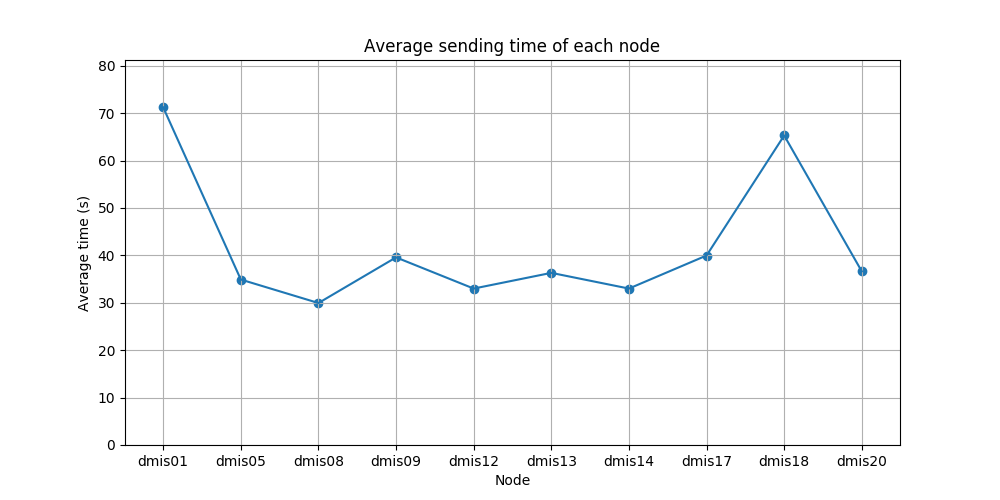
\includegraphics[width=60mm]{images/30/30_avg_snd_duration_ibrdtn}}
    \caption{Durée moyenne d'envoi par nœud (période 30 secondes)}
    \label{fig:30_avg_snd_duration}
\end{figure}

La figure \ref{fig:30_nb_neighbors}, représente le nombre maximal et minimal de voisin(s) par nœud. Nous remarquons une similitude au niveau des minimums comme des maximums. Effectivement, le minimum étant de 1 et le maximum étant situé entre 5 et 8 pour les deux systèmes étudiés.\par

\begin{figure}[h!]
    \centering
    \subfigure[aDTN]{\label{fig:30_nb_neighbors_adtn}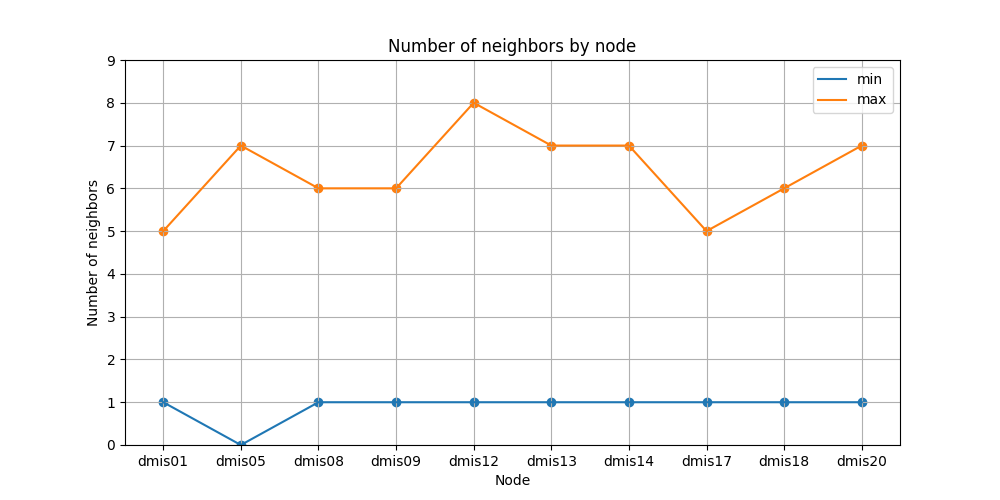
\includegraphics[width=60mm]{images/30/30_nb_neighbors_adtn.png}}
    \subfigure[ibrDTN]{\label{fig:30_nb_neighbors_ibrdtn}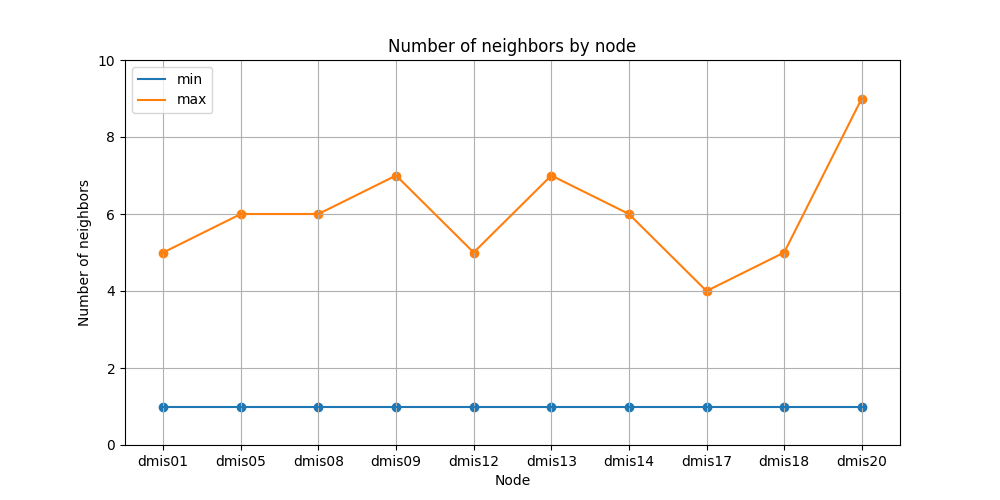
\includegraphics[width=60mm]{images/30/30_nb_neighbors_ibrdtn}}
    \caption{Nombre de voisins par nœud(s) (période 30 secondes)}
    \label{fig:30_nb_neighbors}
\end{figure}

Les diagrammes barres de la figure \ref{fig:30_msg_rcv}, montrent les pourcentages des messages reçus pour chaque nœud. Nous pouvons voir une grande similitude, car les nœuds de aDTN et de ibrDTN, reçoivent quasiment tous 100\% des messages. En revanche, il ne faut pas oublier que du côté de ibrDTN, ces résultats sont biaisés. Ainsi, il faut se référer au nombre exact de messages non reçus qui est de 6 pour aDTN et de 41 pour ibrDTN. Nous remarquons donc que cette fois aDTN est plus efficace que ibrDTN.\par

\begin{figure}[h!]
    \centering
    \subfigure[aDTN]{\label{fig:30_msg_rcv_adtn}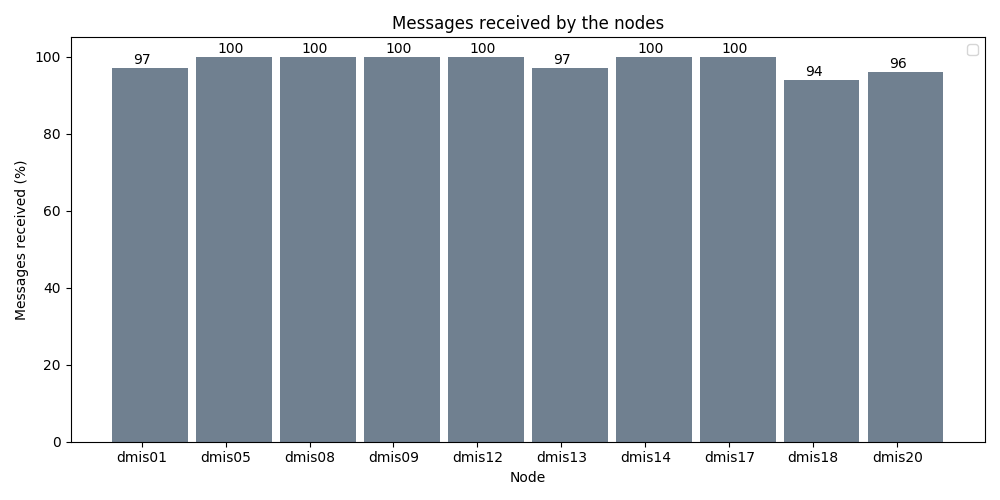
\includegraphics[width=60mm]{images/30/30_msg_rcv_adtn.png}}
    \subfigure[ibrDTN]{\label{fig:30_msg_rcv_ibrdtn}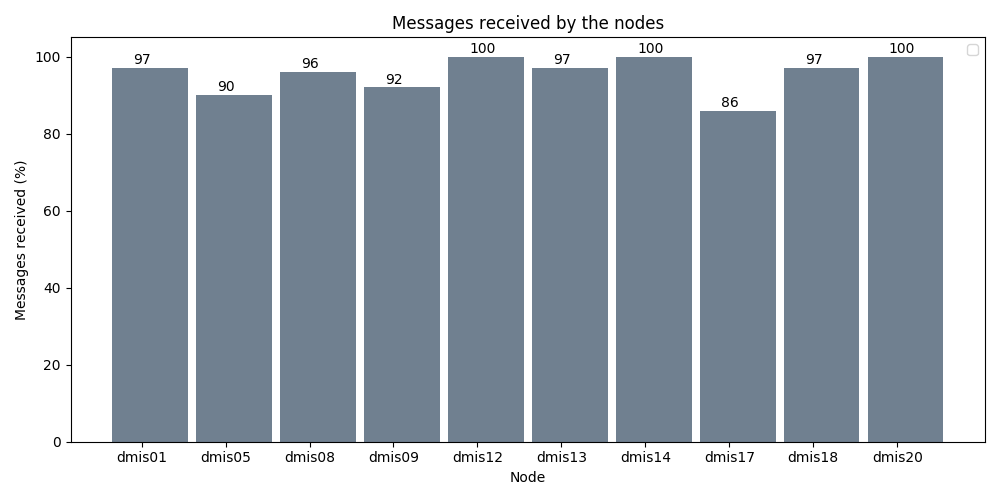
\includegraphics[width=60mm]{images/30/30_msg_rcv_ibrdtn}}
    \caption{Messages reçus par nœud (période 30 secondes)}
    \label{fig:30_msg_rcv}
\end{figure}


\subsection {Période de beaconing : 40 secondes}

Finalement, nous nous sommes intéressés à la recherche de voisin(s) fixée à 40 secondes. Nous remarquons que aDTN reçoit 96\% des messages envoyés alors que ibrDTN en reçoit 93\%. La durée moyenne de réception des messages est de 80 secondes pour aDTN contre 123 secondes pour ibrDTN. Nous pouvons comparer ces moyennes par rapport à la figure \ref{fig:40_avg_rcv_duration} qui présente la durée moyenne de réception des messages par nœud.\par

Sur les graphiques de la figure \ref{fig:40_avg_rcv_duration}, on constate que la durée de réception des messages est majoritairement inférieure à 100 secondes pour aDTN. Concernant le second système, les durées moyennes sont principalement supérieures à 100 secondes. Le nœud dmis01 présente une moyenne plus élevée par rapport aux autres nœuds, pour les deux systèmes. Les durées moyennes de réception sont resserrées dans un intervalle de 50 secondes pour les deux systèmes étudiés (entre 50 et 100 secondes pour aDTN et 100 et 150 pour ibrDTN). \par

\begin{figure}[h!]
    \centering
    \subfigure[aDTN]{\label{fig:40_avg_rcv_duration_adtn}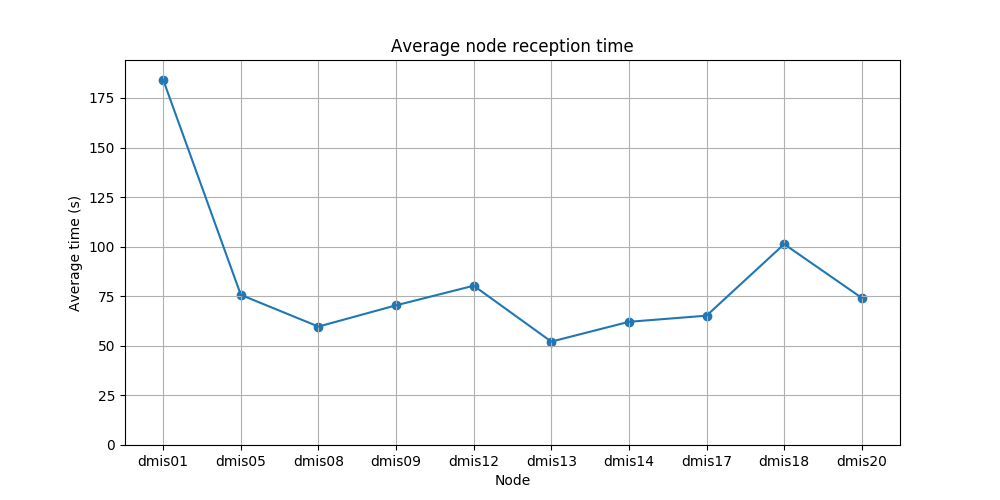
\includegraphics[width=60mm]{images/40/40_avg_rcv_duration_adtn.png}}
    \subfigure[ibrDTN]{\label{fig:40_avg_rcv_duration_ibrdtn}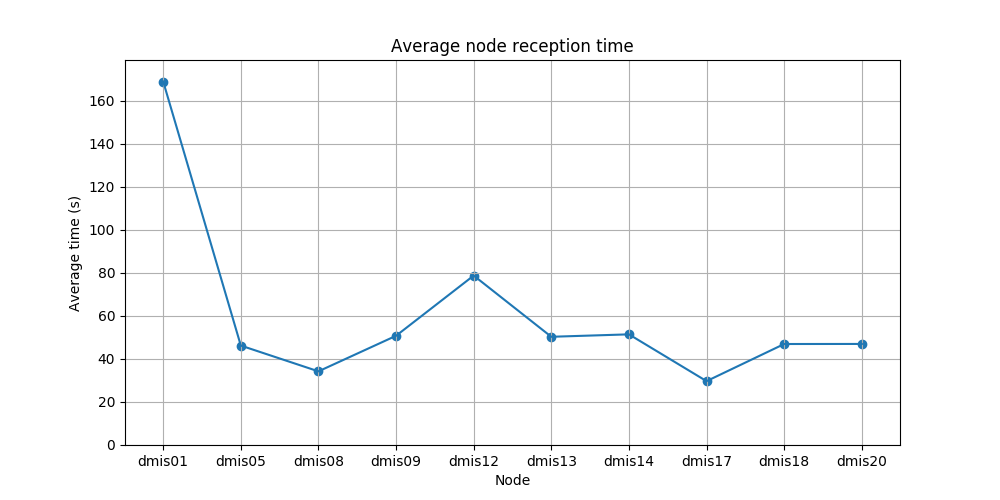
\includegraphics[width=60mm]{images/40/40_avg_rcv_duration_ibrdtn}}
    \caption{Durée moyenne de réception par nœud (période 40 secondes)}
    \label{fig:40_avg_rcv_duration}
\end{figure}
	
D’autre part, il est également intéressant de regarder les résultats de la durée moyenne d'envoi de chaque nœud, en figure \ref{fig:40_avg_snd_duration}. Les résultats montrent que la durée moyenne d'envoi de chaque nœud oscille sur un intervalle compris entre près de 60 à 100 secondes du coté aDTN, avec néanmoins, une durée proche de 120 secondes. En ce qui concerne ibrDTN, l’intervalle se situe entre 75 et 200 secondes. Ainsi, du côté de ibrDTN on a 60\% des moyennes par nœud qui sont à plus de 100 secondes contre 10\% pour aDTN.\par

\begin{figure}[h!]
    \centering
    \subfigure[aDTN]{\label{fig:40_avg_snd_duration_adtn}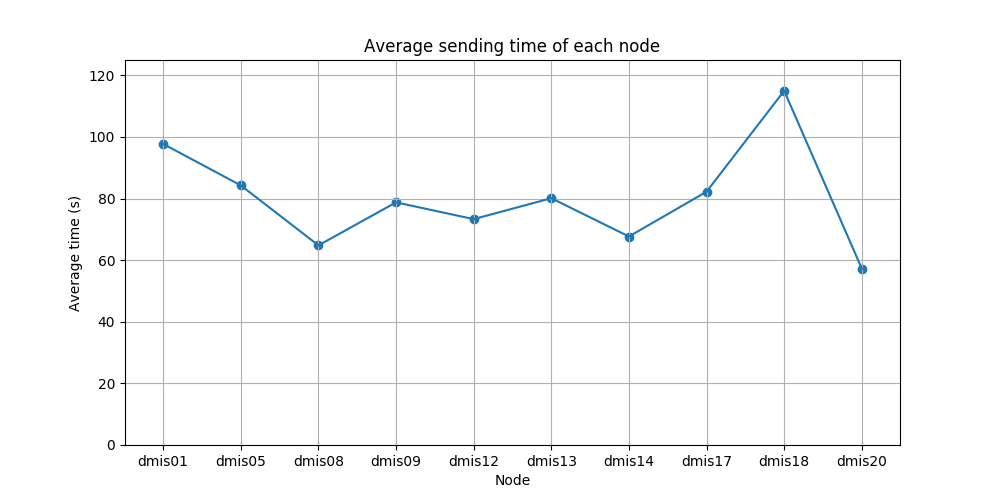
\includegraphics[width=60mm]{images/40/40_avg_snd_duration_adtn.png}}
    \subfigure[ibrDTN]{\label{fig:40_avg_snd_duration_ibrdtn}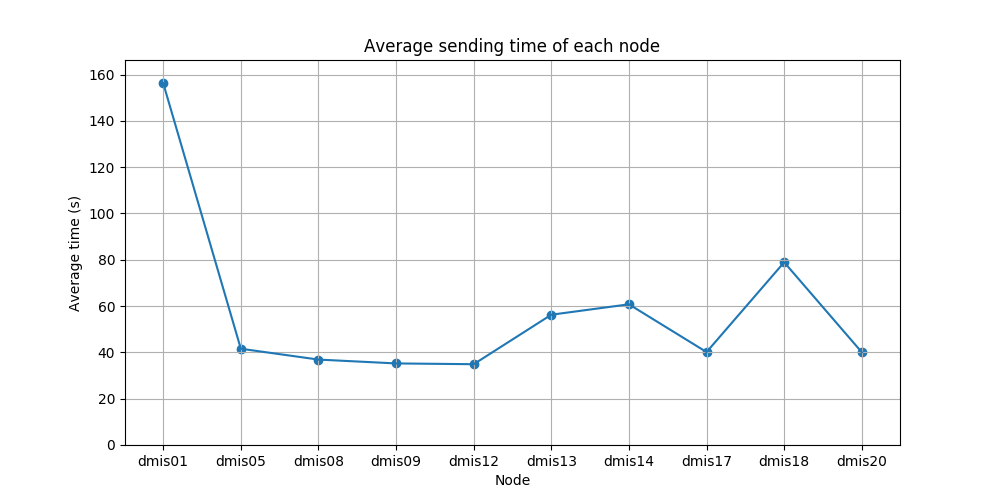
\includegraphics[width=60mm]{images/40/40_avg_snd_duration_ibrdtn}}
    \caption{Durée moyenne d'envoi par nœud (période 40 secondes)}
    \label{fig:40_avg_snd_duration}
\end{figure}

Les courbes de la figure \ref{fig:40_nb_neighbors} présentent le Nombre de voisins par nœud. Celles-ci permettent d'observer que le nombre de voisin(s) minimal est le même pour aDTN et ibrDTN et il est de 1. Le nombre de voisins des nœuds de aDTN est compris entre 5 et 8. Tandis que pour ibrDTN, ce nombre varie entre 4 et 8 voisins.

\begin{figure}[h!]
    \centering
    \subfigure[aDTN]{\label{fig:40_nb_neighbors_adtn}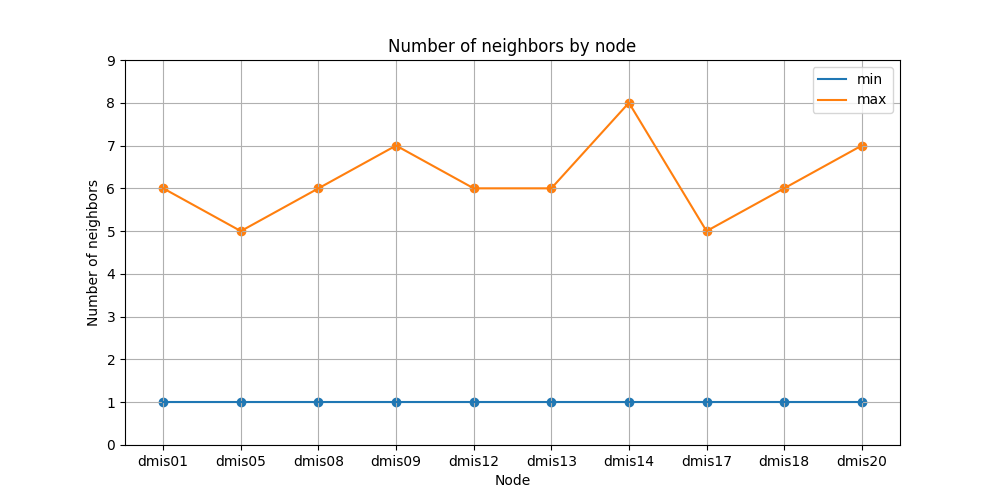
\includegraphics[width=60mm]{images/40/40_nb_neighbors_adtn.png}}
    \subfigure[ibrDTN]{\label{fig:40_nb_neighbors_ibrdtn}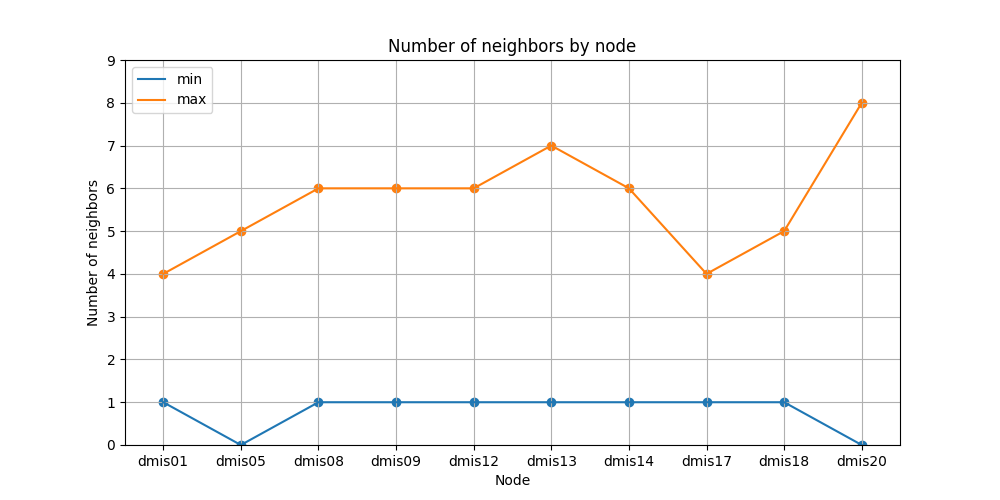
\includegraphics[width=60mm]{images/40/40_nb_neighbors_ibrdtn}}
    \caption{Nombre de voisins par nœud(s) (période 40 secondes)}
    \label{fig:40_nb_neighbors}
\end{figure}

La figure \ref{fig:40_msg_rcv}, affiche les pourcentages des messages reçus pour chaque nœud. Nous pouvons, ainsi, voir une grande similitude, car les nœuds de aDTN reçoivent quasiment 100\% des messages, alors que ceux de ibrDTN reçoivent tous 100\% des messages. Mais, comme expliqué auparavant, ce graphique n’est pas exploitable pour ibrDTN. Par conséquent, nous regardons plutôt le nombre de messages transmis et non reçus. Nous remarquons que ibrDTN n’a pas reçu 31 messages alors que seulement 14 messages ne sont pas arrivés du côté de aDTN, soit moitié moins que ibrDTN.

\begin{figure}[h!]
    \centering
    \subfigure[aDTN]{\label{fig:40_msg_rcv_adtn}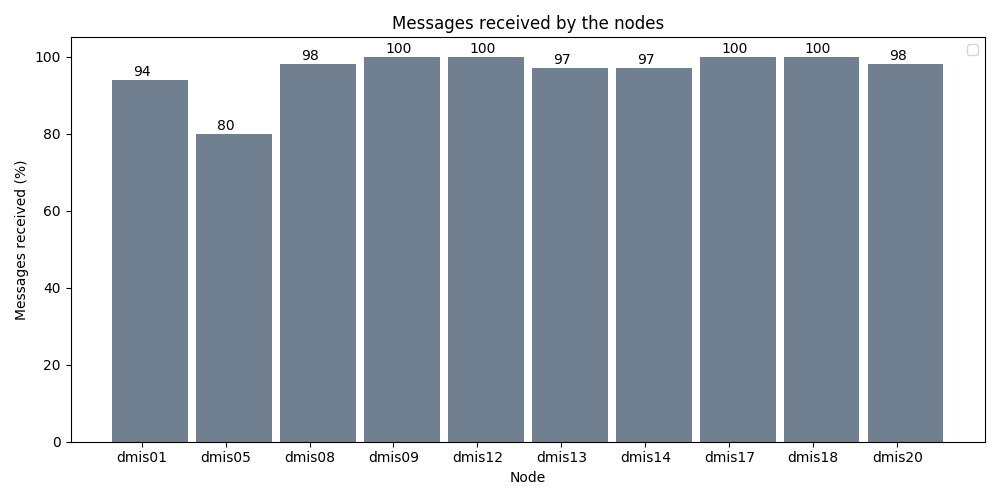
\includegraphics[width=60mm]{images/40/40_msg_rcv_adtn.png}}
    \subfigure[ibrDTN]{\label{fig:40_msg_rcv_ibrdtn}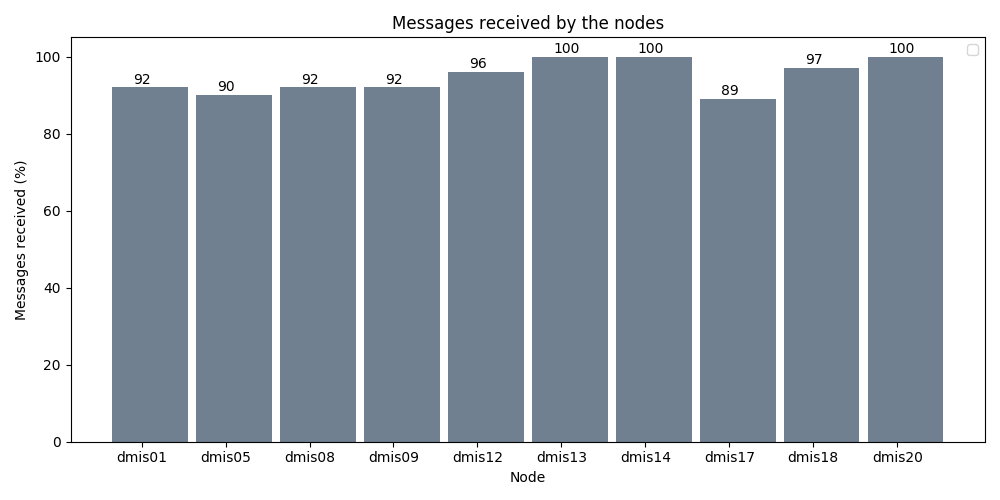
\includegraphics[width=60mm]{images/40/40_msg_rcv_ibrdtn}}
    \caption{Messages reçus par nœud (période 40 secondes)}
    \label{fig:40_msg_rcv}
\end{figure}

%----------------------------------------------------------------------------
\newpage
%----------------------------------------------------------------------------

\section{Conclusion}
Pour conclure, on peut en effet dire que les deux systèmes aDTN et ibrDTN, sont un peu différents. Malgré le fait qu’ils implémentent tous deux le même protocole, ils ont chacun leurs spécificités.\par
En effet, l'étude nous a montré, que aDTN semble être moins performant sur les périodes de découverte de nœuds voisins élevées. Il apparaît au vu des résultats obtenus (figures \ref{fig:05_nb_neighbors_adtn}, \ref{fig:10_nb_neighbors_adtn}, \ref{fig:30_nb_neighbors_adtn} et \ref{fig:40_nb_neighbors_adtn}) que sa recherche de voisins est tout de même quasiment toujours inférieure à celle de ibrDTN. aDTN supporte ainsi beaucoup moins les périodes de découverte de nœuds voisins élevées. En effet, le taux d’envoi de messages est vraiment différent entre une période fixée à 5 secondes et une autre fixée à 30 secondes. Par conséquent, il passe de 23\% de messages envoyés à 96\%, soit un taux de transmission de messages quatre fois plus élevé. Mais, il faut bien noter que les temps de réception des messages avec des périodes élevées sont tout de même intéressants. Ce système met trois fois moins de temps pour réceptionner les messages avec une période élevée, par rapport à une période faible, où il reçoit pratiquement tous les messages. Cela peut tout de même être intéressant si son utilisation autorise beaucoup de perte.\par
Concernant l’implémentation de ibrDTN, elle fait en sorte de supporter une recherche élevée de voisins. Cependant, sa réaction par rapport à des périodes de recherche de voisins faibles, montre une performance moindre. En effet, il reçoit moins de messages lorsque la recherche est faible par rapport à une recherche élevée. Les pourcentages de réception des messages le concernant, le prouve, avec 94\%, 94\%, 90\% et 93\% pour des paramètres respectifs de 5, 10, 30 et 40 secondes.\par
Globalement, ibrDTN obtient de meilleures performances pour des recherches de voisins élevées tandis que aDTN est plus en adéquation avec des recherches de voisins faibles. Ainsi, les deux systèmes sont généralement différents.


%----------------------------------------------------------------------------
\newpage
%----------------------------------------------------------------------------

\bibliographystyle{plain}
\bibliography{references}
\end{document}
